%
% jahr.tex
%
% (c) 2018 Prof Dr Andreas Müller, Hochschule Rapperswil
%
\subsection{Einstrahlung über ein Jahr}
Wir könnten versuchen, die im letzten Abschnitt gefundene Einstrahlung
über einen Tag über ein Jahr zu mitteln.
Allerdings stellt sich dies als nur schwer durchführbar heraus.
Stattdessen wählen wir ein Vorgehen, welches  sich an die 
noch etwas allgmeinere Untersuchung in 
\cite[section 5]{skript:mcgeheelehman}
anlehnt.
Dazu berechnen wir erst die mittlere Insolation auf eine nicht
rotierende und nicht geneigte Kugel im Laufe eines Jahres und
mitteln erst danach über den Tagesgang.

\subsubsection{Nicht drehende Erde}
\begin{figure}%
\centering%
\begin{tikzpicture}[>=latex,thick]
\node at (0,0) {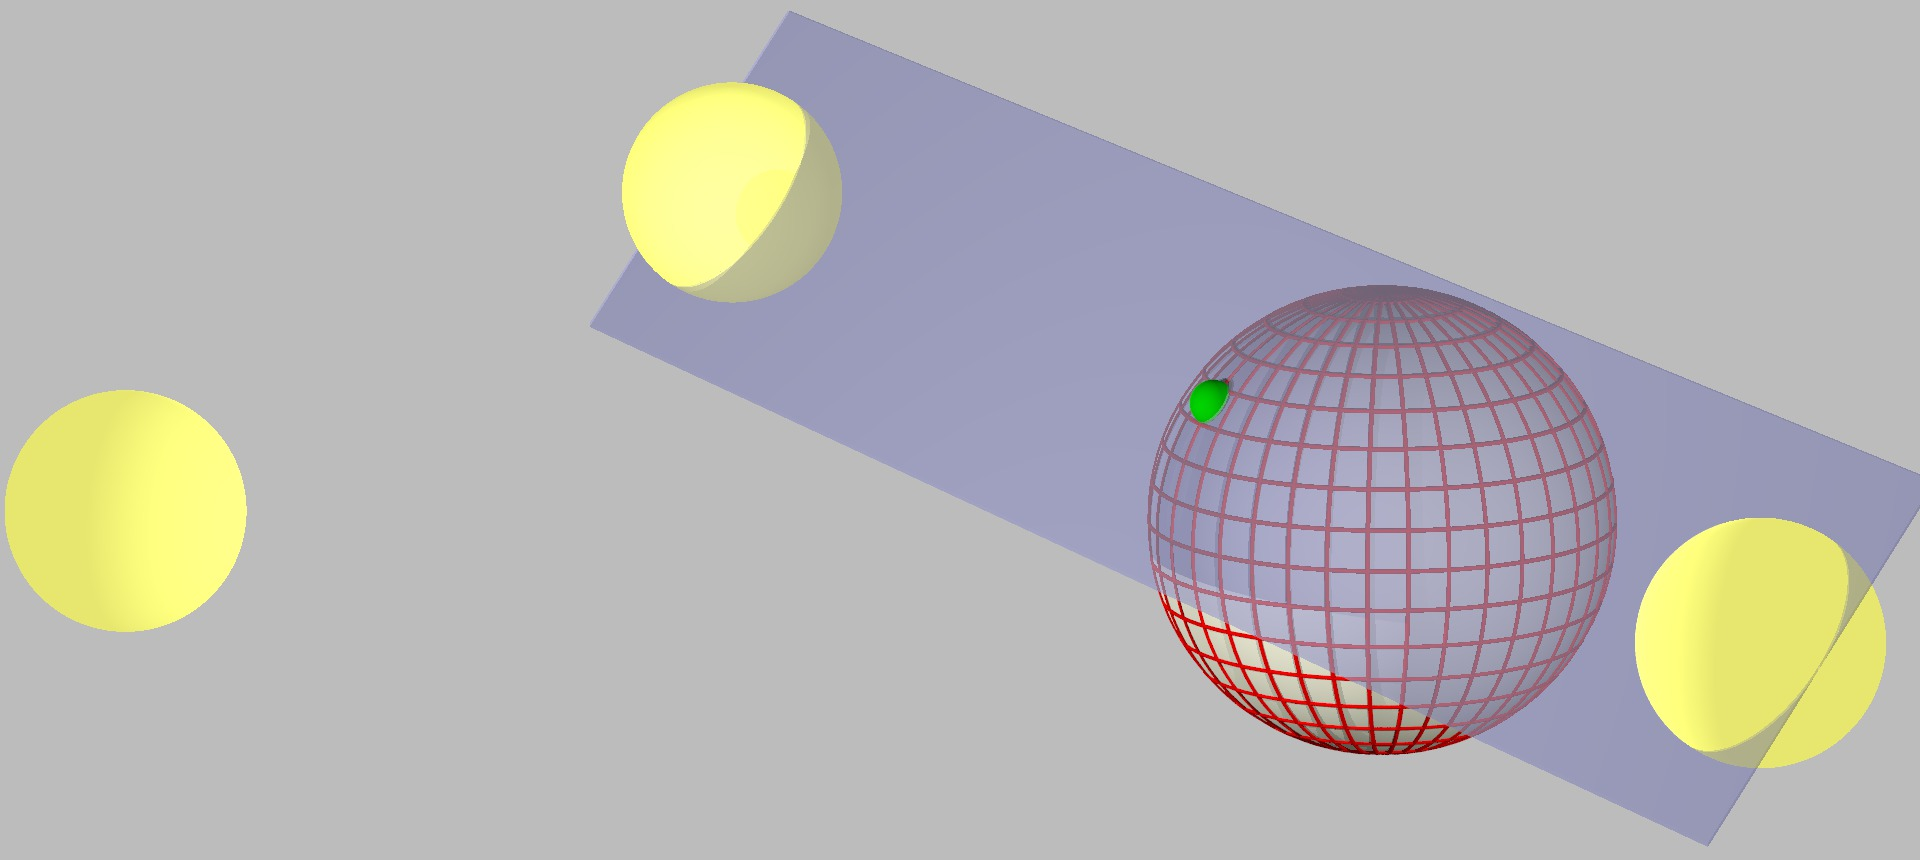
\includegraphics[width=\hsize]{chapters/5/midday.jpg}};
\end{tikzpicture}
\caption{Insolation eines Punktes auf einer nicht geneigten 
und nicht rotierenden Erde im Laufe eines Jahres.
Die Insolation verschwindet, wenn die Sonne sich auf der Tangentialebene
im Punkt befindet, die Insolation ist maximal bei höchster Elevation
der Sonne in der eingezeichneten Position links.
\label{skript:insolation:fest}}
\end{figure}%
Wir betrachten zunächst eine die Sonne auf einer Kreisbahn mit Radius $r$
umlaufende Kugel vom Radius $R$, die sich nicht dreht und gegen die Bahn
nicht geneigt ist.
Wir bezeichnen die Kugel-Koordinaten auf dieser Kugel mit $\hat\vartheta$
und $\hat\varphi$ und wollen die mittlere Insolation
$I(\hat\vartheta,\hat\varphi)$ am Punkt $(\hat\vartheta,\hat\varphi)$
im Laufe eines Jahres berechnen.
Wir nehmen dabei an, dass die Sonne viel weiter entfernt ist als $R$,
also $R\ll r$.
Die Parallaxe des Punktes $(\hat\vartheta,\hat\varphi)$ ist daher
vernachlässigbar.
Da wir ausserdem vo einer Kreisbahn ausgehen, ist das Problem
rotationssymmetrisch um die $z$-Achse, wir können daher annehmen, dass
der Punkt $(\hat\vartheta,\hat\varphi)$ auf dem Nullmeridian liegt,
dass also $\hat\varphi=0$.

Statt die Kugel um die Sonne zu bewegen, können wir die Sonne auch
im Laufe eines Jahres gleichmässig um den Punkt $(\hat\vartheta,\hat\varphi)$
bewegen.
Wir drücken dies dadurch aus, dass der Punkt Strahlung aus der Richtung
$(\cos\lambda,\sin\lambda,0)$ erhält, $\lambda$ ist die Länge der Position
der Sonne.
Natürlich erhält der Punkt nur Strahlung, wenn die Sonne über dem lokalen
Horizont ist.
Für einen Punkt auf dem Nullmeridian bedeutet dies, dass
$-\frac{\pi}2\le \lambda \le \frac{\pi}2$ sein muss.
Diese Situation ist in Abbildung~\ref{skript:insolation:fest} 
dargestellt.

Die mittlere Insolation auf den Punkt $(\hat\vartheta,0)$ ist dann
\begin{align*}
I(\hat\varphi,0)
=
\frac{S_0}{2\pi}
\int_{-\frac{\pi}2}^{\frac{\pi}2}
\begin{pmatrix}
\cos\lambda\\\sin\lambda\\0
\end{pmatrix}
\cdot
\begin{pmatrix}
\sin\hat\vartheta\\0\\\cos\hat\vartheta
\end{pmatrix}
\,d\lambda
=
\frac{S_0}{2\pi}
\int_{-\frac{\pi}2}^{\frac{\pi}2}
\cos\lambda\sin\hat\vartheta\,d\lambda
=
\frac{S_0}{\pi} \sin\hat\vartheta.
\end{align*}
Darin ist $S_0$ der Strahlungsfluss ausserhalb der Erdatmosphäre.
Offenbar hängt die Insolation nur von $\sin\hat\vartheta$ ab.
Wir können dies auch durch die $z$-Koordinate ausdrücken, es
ist nämlich
\begin{equation}
\sin\hat\vartheta = \sqrt{1-\cos^2\hat\vartheta}=\sqrt{1-z^2}.
\label{skript:einstrahlung:sintheta}
\end{equation}

\subsubsection{Geneigte Erde}
Um die Insolation auf einen Punkt auf der geneigten Erde zu ermitteln
brauchen wir die Umrechnung von Koordinaten $(\vartheta,\varphi)$ 
in die geographische Breite in dem Koordinatensystem, welches im
vorangegangenen Abschnitt als Basis diente.
Die Drehmatrix
\[
D_\gamma
=
\begin{pmatrix}
\cos\gamma&0&-\sin\gamma\\
0&1&0\\
\sin\gamma&0&\cos\gamma
\end{pmatrix}
\]
dreht einen Punkt auf der Kugeloberfläche um den Neigungswinkel
$\gamma$ der Erde.
Wir erhalten für den Punkt $(\vartheta,\varphi)$
\[
D_\gamma\begin{pmatrix}
\sin\vartheta\cos\varphi\\
\sin\vartheta\sin\varphi\\
\cos\vartheta
\end{pmatrix}
=
\begin{pmatrix}
\cos\gamma\sin\vartheta\cos\varphi -\sin\gamma\cos\vartheta\\
\sin\vartheta\sin\varphi\\
\sin\gamma\sin\vartheta\cos\varphi + \cos\gamma\cos\vartheta
\end{pmatrix}.
\]
Davon brauchen wir nur die letzte Koordinate, es ist
\begin{equation}
\cos\hat\vartheta
=
\sin\gamma\sin\vartheta\cos\varphi+\cos\gamma\cos\vartheta.
\end{equation}
Auf der nicht rotierenden aber geneigten Erde ist die Insolation
im Punkt $(\vartheta,\varphi)$ also
\begin{equation}
I(\vartheta,\varphi)
=
\frac{S_0}{\pi}
\sin\hat\vartheta
=
\frac{S_0}{\pi}
\sqrt{1-
(\sin\gamma\sin\vartheta\cos\varphi+\cos\gamma\cos\vartheta)^2}.
\label{skript:chapter:inspunkt}
\end{equation}

\subsubsection{Mittelung über einen Tag}
\begin{figure}
\centering
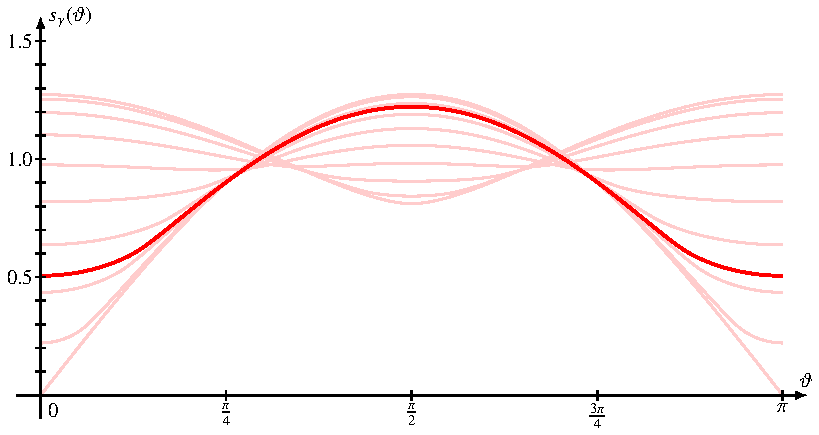
\includegraphics{chapters/5/ell2.pdf}
\caption{Mittlere Insolation über ein Jahr in Abhängigkeit von der
geographischen Breite.
Die hellroten Kurven zeigen die Insolation für Achsneigungen zwischen
$0^\circ$ ($\sin\theta$-Kurve mit Nullstellen an den Intervallenden)
und $90^\circ$.
\label{skript:einstrahlung:jahrinsbild}}
\end{figure}
Jetzt müssen wir die Insolation noch über die Rotation im Laufe eines 
Tages mitteln.
Wir erreichen dies, indem wir \eqref{skript:chapter:inspunkt}
über $\varphi$ über eine volle Umdrehung mitteln:
\begin{align}
I(\vartheta)
&=
\frac{1}{2\pi}
\int_0^{2\pi}
\frac{S_0}{\pi}
\sqrt{1-
(\sin\gamma\sin\vartheta\cos\varphi+\cos\gamma\cos\vartheta)^2}
\,d\varphi
\notag
\\
&=
\frac{S_0}{2\pi^2}
\int_0^{2\pi}
\sqrt{1-
(\sin\gamma\sin\vartheta\cos\varphi+\cos\gamma\cos\vartheta)^2}
\,d\varphi.
\label{skript:einstrahlung:mittlereinsolation}
\end{align}
Das Integral auf der rechten Seite ist nicht in geschlossener
Form lösbar.
Die numerische Berechnung mit Octave ergibt den Graphen
in Abbildung~\ref{skript:einstrahlung:jahrinsbild}.

Als Spezialfall sei notiert, dass im Falle verschwindender Neigung
$\gamma=0$ das Integral zu
\begin{align*}
I(\vartheta)
&=
\frac{S_0}{2\pi^2}
\int_{-\frac{\pi}2}^{\frac{\pi}2}
\sqrt{1-\cos^2\vartheta}
\,d\varphi
=
\frac{S_0}{2\pi^2}
\int_{-\frac{\pi}2}^{\frac{\pi}2}
\sin\vartheta
\,d\varphi
=
\frac{S_0}{\pi}
\sin\vartheta
\end{align*}
wird.
In Abbildung~\ref{skript:einstrahlung:jahrinsbild} ist dies die
Kurve mit den Nullstellen an den Intervalenden.
Man erkennt auch, dass im Spezialfall $\gamma=90^\circ$ die Insolation zu
\begin{align*}
I(\vartheta)
&=
\frac{S_0}{2\pi^2}
\int_{-\frac{\pi}2}^{\frac{\pi}2}
\sqrt{1- \sin^2\vartheta\cos^2\varphi}
\,d\varphi
\end{align*}
wird.
Man kann ablesen und sieht dies auch in der 
Abbildung~\ref{skript:einstrahlung:jahrinsbild} bestätigt, dass
die mittlere Insolation am Äquator ist als an den Polen.
Wenn nämlich $\sin\vartheta_1 < \sin\vartheta_2$, dann ist
\begin{align*}
\sqrt{1- \sin^2\vartheta_1\cos^2\varphi}
&>
\sqrt{1- \sin^2\vartheta_2\cos^2\varphi}
\\
\Rightarrow
\qquad
\frac{S_0}{2\pi^2}
\int_{-\frac{\pi}2}^{\frac{\pi}2}
\sqrt{1- \sin^2\vartheta_1\cos^2\varphi}
\,d\varphi
&>
\frac{S_0}{2\pi^2}
\int_{-\frac{\pi}2}^{\frac{\pi}2}
\sqrt{1- \sin^2\vartheta_2\cos^2\varphi}
\,d\varphi,
\end{align*}
in der Mitte des Intervals bei $\vartheta=\frac{\pi}2$ ist $I(\vartheta)$
daher minimal.

